\documentclass[a4paper, 11pt]{article}
\usepackage[text={170mm, 240mm}, left=20mm, top=30mm]{geometry}
\usepackage[utf8]{inputenc}
\usepackage[czech]{babel}
\usepackage{times}
\usepackage[dvipsnames]{xcolor}
\usepackage{graphicx}
\usepackage{hyperref}

\begin{document}
\begin{titlepage}
\vspace*{\fill}
\noindent {\fontsize{65}{50} \color{ForestGreen} \textsc{Calc-chan}} {\Large \textsc{by Paks}}\\[0.3em]
{\fontsize{40}{40}\textsc{Uživatelský manuál}}
\vspace*{\fill}
\end{titlepage}
	
\tableofcontents

\newpage

\section{Úvod}
Calc-chan je jednoduchá aplikace pro vyhodnocování jednoduchých matematických výrazů. Mezi matematické funkce, které Calc-chan nabízí patří sčítání, odčítání, násobení, dělení, mocnina, obecná odmocnina, faktoriál a přirozený logaritmus.

\section{Prerekvizity}
Aplikace byla vyvinuta v programovacím jazyce Python3 a pro grafické rozhraní využívá také knihovnu Python3 tkinter. Instalátor však tento problém řeší za uživatele a prerekvizity nainstaluje sám.

\section{Instalace a spuštění}
K nainstalování aplikace Calc-chan je potřeba stáhnout instalátor \texttt{\textbf{cchan.deb}}. \\

\noindent Po stažení instalátoru a po přesunu do adresáře ve kterém se nachází je možné instalátor spustit následujícím příkazem:\\
\texttt{\textbf{sudo apt install ./cchan.deb}}\\

\noindent Alternativně je možné se do stejného adresáře přesunout skrze průzkumníka a instalátor spustit dvojím kliknutím na instalátor. Zobrazí se okno s informacemi o aplikaci a možností instalace.\\

\noindent Po instalaci je možné aplikaci Calc-chan spustit z libovolného adresáře příkazem \texttt{\textbf{cchan}}.

\section{Vzhledy}
Calc-chan nabízí uživateli výběr ze dvou barevných motivů -- světlého a tmavého. Motiv se dá změnit v kontextovém menu po kliknutí na tlačítko \texttt{Barva motivu}.\\
\begin{center}
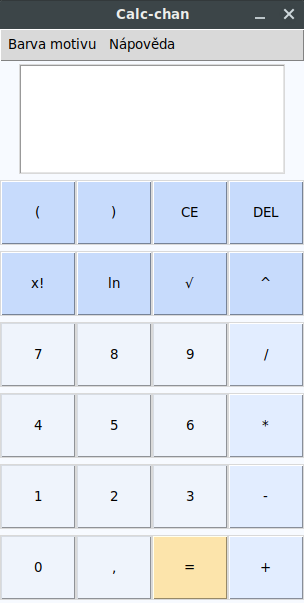
\includegraphics[scale=0.5]{screenshot.png}
\hspace{50pt}
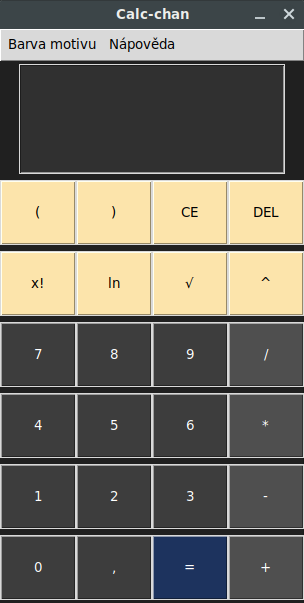
\includegraphics[scale=0.5]{screenshot2.png}
\end{center}



\end{document}